\documentclass{article}
\usepackage[english]{babel}
\usepackage[utf8]{inputenc}
\usepackage{johd}
\usepackage{geometry}
\geometry{a4paper, margin=1in}
\usepackage{graphicx} 
\usepackage{float}
\usepackage{cite}
\usepackage{setspace}
\usepackage{hanging}
\usepackage{titling}
\usepackage{indentfirst}


\title{The Optimization of Flight Routes: Enhancing Efficiency and Maximizing Profitability}

\author{Ian R. Wald\\
        \small Institute for Computing in Research\\
        \small Santa Fe, New Mexico}

\date{July 31st, 2024}

\begin{document}

\maketitle

\begin{abstract} 
\noindent This research paper presents a simulation model designed to optimize flight routes across the continental United States by evaluating various metrics, including flight time, operational cost, maintenance cost, and net profit. The model generates and visualizes a range of flight paths, containing direct routes as well as those with one or two stops. By systematically assessing these routes, the study identifies and addresses levels of optimizations and what factors are needed to change and enhance overall route efficiency and profitability. The findings are expected to provide valuable insights for airlines seeking to streamline operations and improve financial performance through data-driven route optimization strategies. \\
 \end{abstract}
\noindent\keywords\textit{flight route optimization; simulation model; operational efficiency;     
 profitability analysis; route planning}
 
\section{Introduction}

Efficient flight route management is crucial for the aviation industry, where operational costs and profitability are tightly interlinked with route planning. Traditional methods of route optimization often rely on historical data and static models, which may not fully account for dynamic changes in operational conditions or emerging efficiencies. This research paper explores a novel simulation approach that generates and visualizes a variety of hypothetical flight routes across the continental United States. By incorporating metrics such as flight time, operational and maintenance costs, and net profit, the model aims to provide a comprehensive evaluation of route performance.
The primary objective of this study is to identify and replace inefficient routes with more effective alternatives, thereby optimizing overall route efficiency. The simulation evaluates direct routes and those with one or two stops, offering a comparative analysis of each route’s impact on operational and financial outcomes. Through this approach, the research seeks to provide actionable insights for airlines and route planners, enabling them to make data-driven decisions that enhance route profitability and operational efficiency.

\section{Background}

Since the inception of the commercial aviation industry in 1914, the landscape of domestic air travel in the United States has evolved dramatically. From the pioneering days of a single-passenger flight between St. Petersburg and Tampa, Florida, the industry has expanded to manage over 45,000 flights daily. This exponential growth reflects advancements in aircraft technology, increased accessibility, and a rising demand for air travel. The robust network of domestic flights has necessitated sophisticated route planning to accommodate the volume and complexity of modern air traffic while ensuring safety and efficiency.\\

The journey from early aviation to today's bustling skies has been marked by numerous milestones. The introduction of jet engines, deregulation in the late 1970s, and the rise of low-cost carriers have all contributed to making air travel more affordable and accessible to the masses. These changes have not only increased passenger numbers but also intensified competition among airlines, pushing them to optimize operations and maximize efficiency. The growth of major hubs and the development of airports have further facilitated the expansion of domestic air travel, creating a comprehensive and interconnected network that serves millions of passengers annually.\\

Route optimization has traditionally relied on historical data and established patterns to determine flight paths. These static models, while effective to a degree, often fail to account for the dynamic nature of the aviation environment, where operational conditions can change rapidly due to weather, air traffic control restrictions, and varying fuel costs. Additionally, calculating the precise distances between various waypoints is crucial for accurate route planning. The Haversine formula, which computes the shortest distance between two points on the Earth's surface, is essential in this context. It allows airlines to determine the most efficient routes by providing accurate distance measurements, thereby playing a critical role in optimizing flight paths.\\

Recent technological advancements have paved the way for innovative simulation models that offer a more holistic and dynamic approach to route optimization. By integrating real-time data and sophisticated algorithms, these models can generate a wide range of hypothetical flight paths, including direct routes and those with intermediate stops. The Haversine formula is used extensively in these models to calculate accurate distances between various points, ensuring that the generated routes are both realistic and efficient. This simulation-based approach allows for a detailed evaluation of each route's impact on key performance metrics, such as flight time, operational and maintenance costs, and overall profitability. The ability to visualize and compare these routes provides valuable insights for airlines, enabling them to identify inefficiencies and implement data-driven strategies to enhance route performance and financial outcomes.

\section{Methods}
\subsection*{Generation of Initial Flights}
To simulate various hypothetical flight routes across the continental United States, a Python program was developed to generate all possible flights from a predefined set of airports. This initial step involved creating a dataset of potential routes, including direct flights and those with one or two layovers. The program calculated essential metrics for each route, such as total distance, flight time, operational and maintenance costs, layover time, number of passengers, and net profit. The Haversine formula was employed to determine distances between geographic coordinates, while a simulation model accounted for layover impacts. The generated flight data were compiled into a comprehensive dataset, stored in a text file (\texttt{generated\_flights\_new.txt}), for subsequent analysis and optimization. 

\subsection*{Optimization of Flight Routes: Sequencing of Stops}
\begin{figure}[h!] 
\centering
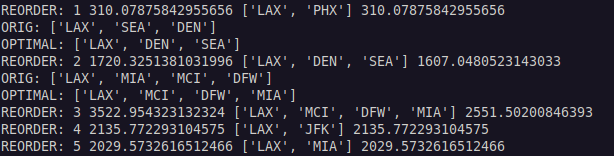
\includegraphics[width=\textwidth]{images/sorting_alg.png}
\caption{Route Optimization Comparison: The chart contrasts the original (ORIG) and optimized (OPTIMAL) routes, including reordering sequence, previous distance, airport order, and new distance.}
\label{fig:sorting}
\end{figure}

Following the generation of flights, a separate program optimized the flight paths by reordering them to minimize the total distance traveled. This was accomplished by parsing the flight data from the generated text file and extracting information such as flight number, origin, destination, stops, and coordinates. Using the Haversine formula, the program calculated the great-circle distance between waypoints and reordered the stops to create more efficient flight routes. Performance metrics were recalculated for the optimized routes. The optimized data were then written to a new output file (\texttt{sorted\_flights\_new.txt}), providing a refined dataset for further processing.\\
\\
\subsection*{Identification and Replacement of Unprofitable Flights}
After optimizing the flight paths, further optimization was needed. A program focused on identifying and eliminating unprofitable routes. Using a predefined profit threshold, the program categorized flights into profitable and eliminated groups. For each eliminated flight, the program identified the closest profitable flight path using a cumulative distance metric, minimizing the distance between cities on the eliminated path and those on the profitable paths. This process ensured that passengers from unprofitable flights were rerouted to the most similar and convenient alternatives available. 

\begin{figure}[H]
\centering
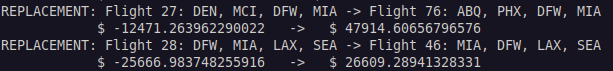
\includegraphics[width=\textwidth]{images/replacement.png}
\caption{Flight Replacement for Profit Maximization. This figure compares the net profits of the original and new flights.}
\label{fig:replacement}
\end{figure}

The program also accommodated passengers from eliminated flights onto replacement flights, ensuring that the number of passengers did not exceed the aircraft's maximum capacity of 204. The updated profitable flight paths, including the new passenger counts, were saved to a file (\texttt{profitable\_flights.txt}), reflecting the loss of flights but resulting in an optimized and more profitable flight schedule for the airline. 

\subsection*{Visualization and Analysis}

\begin{figure}[H] 
\centering

% Top image
\begin{minipage}{\textwidth}
    \centering
    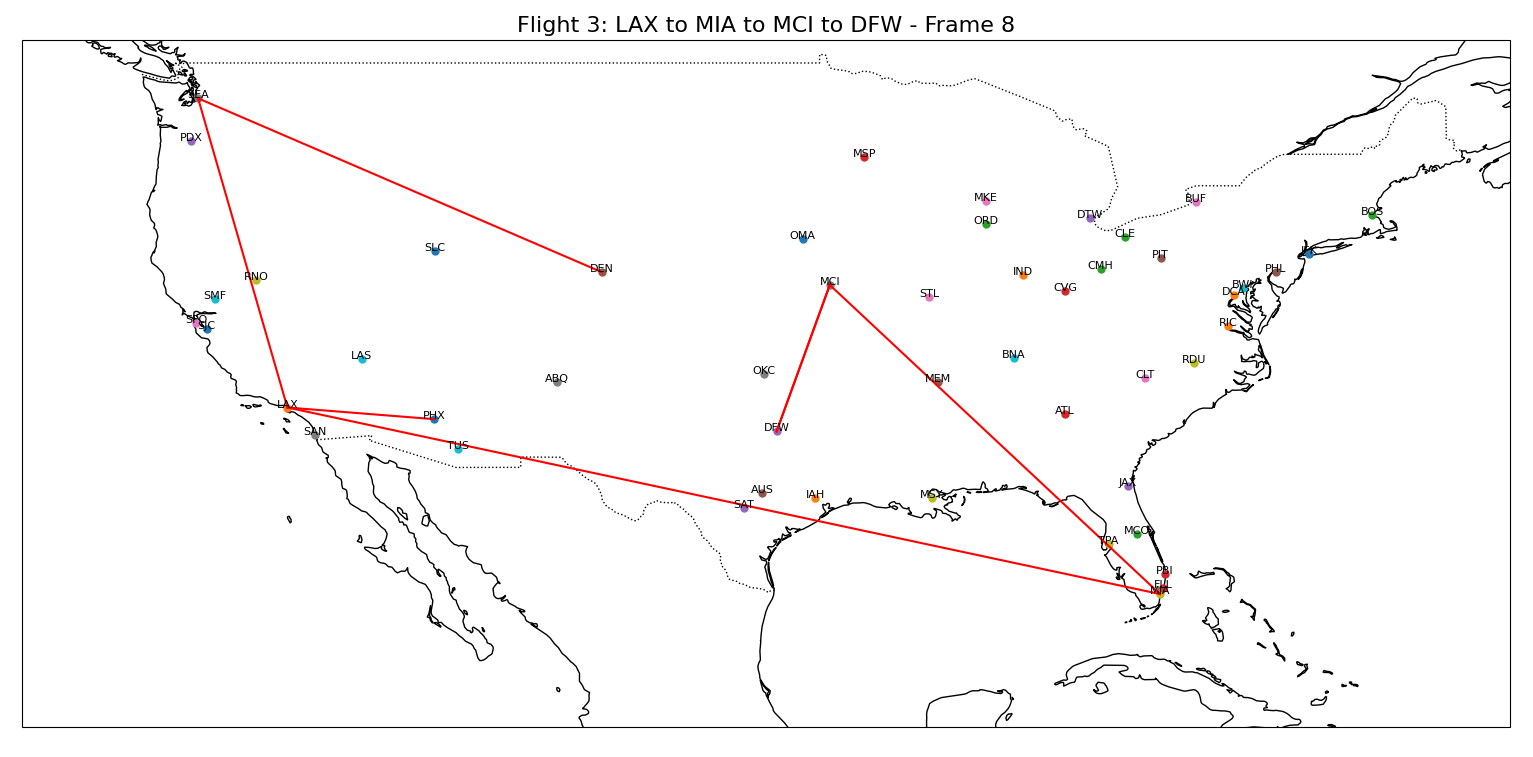
\includegraphics[width=\textwidth]{images/unsort_vis.png}
    \caption{Before Sorting—First 3 Flights.}
    \label{fig:top}
\end{minipage}

\end{figure}

To visualize the outputs and understand how the flight routes would look in the continental United States, an animation of the flight paths and their level of optimization was created, as shown in Figures~\ref{fig:top} (See Above) and \ref{fig:bottom} (See on Next Page). This provided an intuitive understanding of the changes made to the flight routes and their impact on efficiency. Additionally, a bar graph comparing variables such as total net profit, total passenger miles, and total passengers across all three output files was generated, enabling a thorough evaluation and identification of trends. The effectiveness of each optimization state is demonstrated by enhancing route efficiency and profitability.

% Bottom image
\begin{figure}[H] 
\centering

\begin{minipage}{\textwidth}
    \centering
    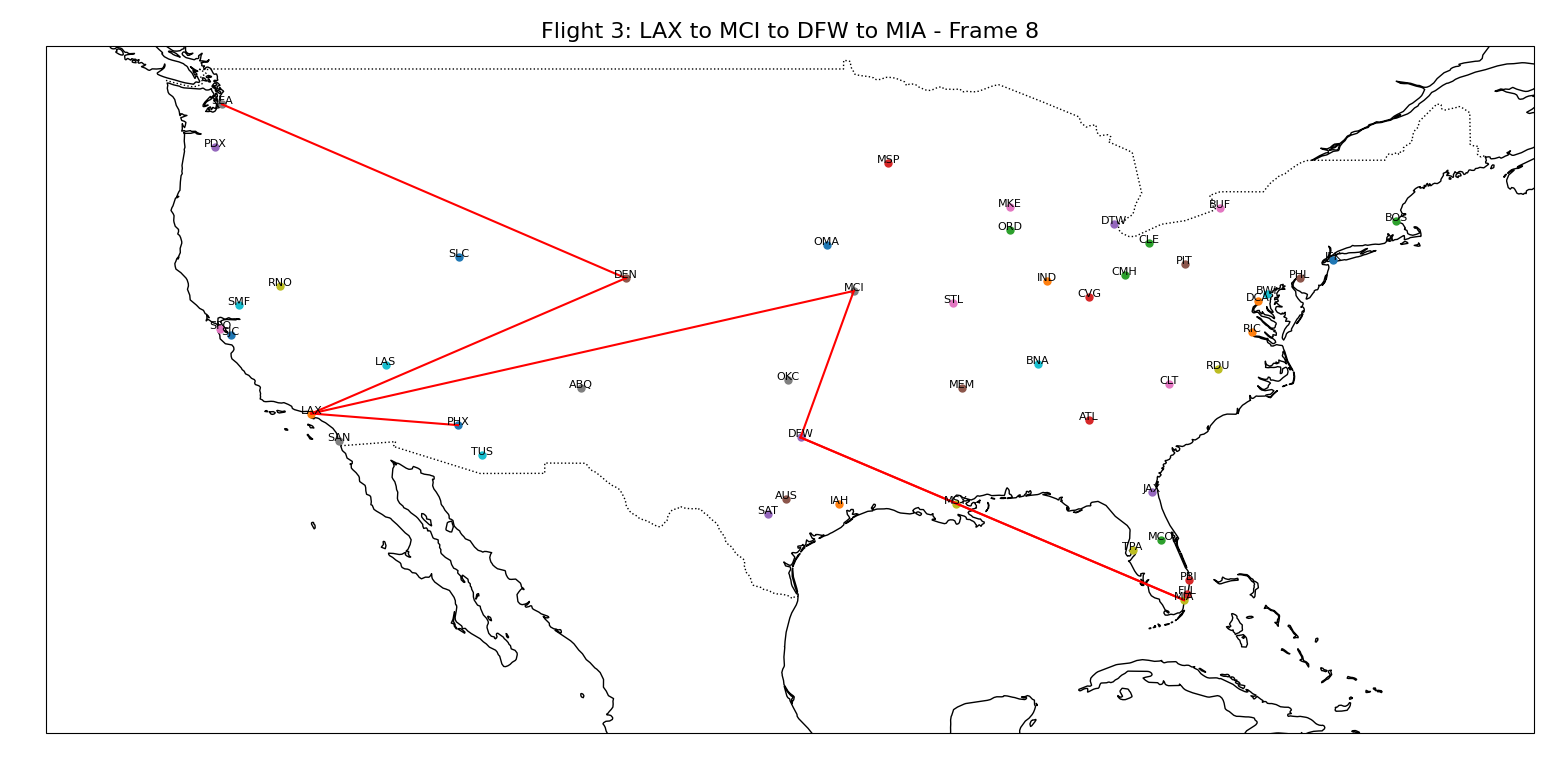
\includegraphics[width=\textwidth]{images/sort_vis.png}
    \caption {After Sorting—First 3 Flights.}
    \label{fig:bottom}
\end{minipage}

\end{figure}

\section{Results}

\begin{figure}[H] 
\centering

\begin{minipage}{\textwidth}
    \centering
    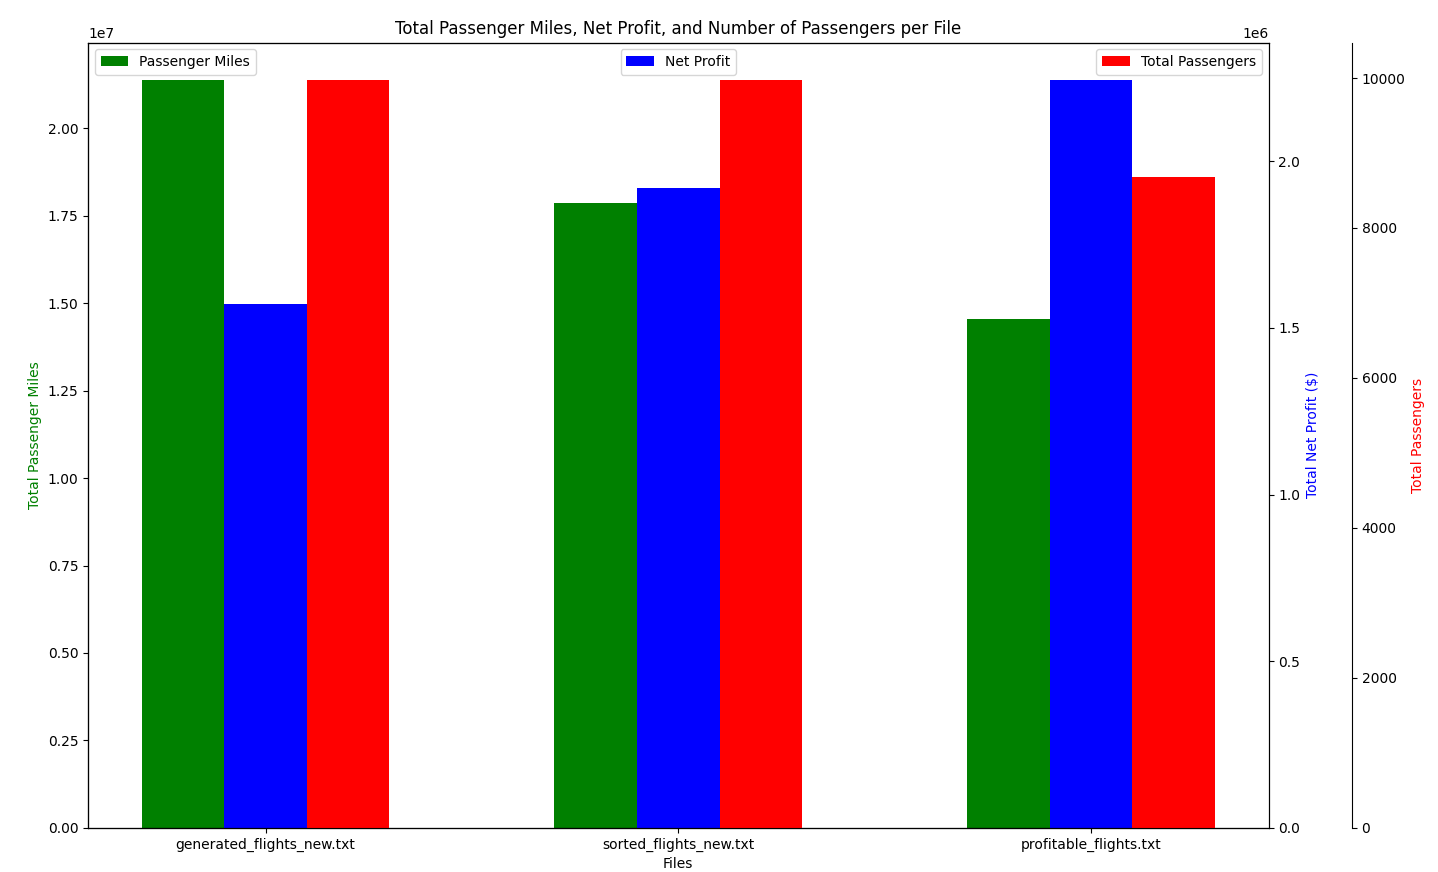
\includegraphics[width=\textwidth]{images/Figure_1.png}
    \caption {Bar graph displaying the totals for passenger miles, net profit, and passengers across all three optimization layers}
\end{minipage}

\end{figure}

With an examination of the graph, it presents the comparative analysis of three different optimization approaches for flight routes— "\texttt{generated\_flights\_new.txt}," "\texttt{sorted\_flights\_new.txt}," and "\texttt{profitable\_
flights.txt}" —by evaluating their performance in terms of total passenger miles, net profit, and total passengers. Each bar represents a different metric, with passenger miles in green, net profit in blue, and total passengers in red. This visualization aids in understanding the impact of each optimization strategy on the airline's operational and financial metrics.\\

In the "\texttt{generated\_flights\_new.txt}" dataset, the figure observes a strong performance in total passenger miles, indicating that this approach effectively covers long distances. However, its net profit and total passenger numbers are comparatively lower. This suggests that this method ensures extensive travel coverage, but may not be the most profitable or passenger-dense option. This stage of optimization involves the initial generation of all possible flight routes from a predefined set of airports, including direct flights and those with layovers. Despite the comprehensive coverage, the generated flights reflect a lower profitability and passenger volume, highlighting potential inefficiencies and underutilized routes.\\

The "\texttt{sorted\_flights\_new.txt}" dataset shows a balanced and impressive performance across all metrics. It achieves high values in total passenger miles, net profit, and total passengers, making it a robust approach. This stage focuses on sequencing stops to minimize the total distance traveled, which is achieved by reordering flight paths using the Haversine formula to calculate great-circle distances. The refined dataset from this optimization results in a significant improvement in both financial and operational metrics, indicating a more efficient allocation of resources and better route planning.\\

For the "\texttt{profitable\_flights.txt}" dataset, the graph showcases the highest net profit, demonstrating that this optimization is particularly effective in financial terms. However, it records lower values for total passenger miles and total passengers. This stage involves identifying and eliminating unprofitable routes and replacing them with the closest profitable flight paths, ensuring that passengers are rerouted to the most convenient alternatives. This results in a reduction in the total number of flights but maximizes profitability. The decrease in passenger miles and numbers reflects the consolidation of routes to focus on high-yield paths, thus enhancing financial outcomes at the expense of overall coverage and passenger volume.

\section{Discussion}

The different trends observed in each dataset highlight the various impacts of the optimization strategies employed. The "\texttt{generated\_flights\_new.txt}" dataset, with its high passenger miles but lower profitability and passenger numbers, indicates an extensive but less efficient initial flight generation. The "\texttt{sorted\_flights\_new.txt}" optimization shows that reordering stops can significantly enhance both profitability and passenger numbers while maintaining high passenger miles, suggesting a balanced and effective approach to route optimization.
The "\texttt{profitable\_flights.txt}" dataset, while achieving the highest net profit, demonstrates the trade-off between financial optimization and overall passenger service. The reduction in total flights and the subsequent impact on passenger miles and numbers underscore the focus on eliminating unprofitable routes and concentrating on high-revenue flights. This strategy, though financially beneficial, may limit the airline's coverage and capacity to serve a larger passenger base.
The comparative analysis of these datasets provides valuable insights into the effectiveness of different optimization strategies. The initially generated flights offer a broad perspective of potential routes, but with inefficiencies that affect profitability and passenger volumes. The sorting optimization enhances route efficiency by minimizing travel distances and improving overall metrics. The final stage, focusing on profitability, underscores the importance of financial performance but also highlights the necessity of balancing it with operational efficiency and passenger service. 

\section{Possible Errors}

Several potential errors could affect the accuracy and effectiveness of the flight optimization process due to the simplified nature of the model and the constraints imposed by the problem's parameters. The reliance on the Haversine formula, which assumes a spherical Earth, may introduce minor inaccuracies, particularly for long-haul flights where more precise models are needed. The simulation also simplifies real-world scenarios by treating intermediate stops as part of a single flight path, whereas in practice, these would be separate flights with distinct operational dynamics. This simplification, combined with the fixed cap of 204 passengers for accommodation, may not accurately reflect real-world constraints and capacity limits. Moreover, the need to distill complex factors into a more manageable model means that multiple variables, such as variations in flight speeds, operational costs, and layover times, are approximated or standardized, potentially affecting the reliability of the profitability assessments and optimization results.\\
\\

\section{Conclusions}

The flight optimization methodology proved effective in enhancing route efficiency by minimizing travel distances and recalculating performance metrics, which likely led to increased profitability. By systematically identifying and eliminating unprofitable flights and finding geographically and economically viable replacements, the approach minimized disruption while optimizing profitability. The accommodation of passengers from eliminated flights, though capped, demonstrated a practical method for managing passenger rerouting. Visualization tools and detailed data analysis provided clear insights into the improvements achieved, confirming the effectiveness of the optimization process. Future efforts should focus on refining distance calculations, improving data accuracy, exploring more sophisticated optimization algorithms, and incorporating real-world constraints for a more comprehensive and practical approach.

\section{Acknowledgements}

I would like to express my gratitude to my mentor, Ed Fenimore for his invaluable support, assistance, and insight as he was instrumental in navigating the complexities of this project. Additionally, I extend my thanks to the Institute for Computing in Research for their resources and support. Special thanks are also due to Rhonda Crespo and Mark Galassi for their encouragement and contributions.

\newpage

\section*{\centering References}

\begin{enumerate}
    \item Federal Aviation Administration. (n.d.). \textit{Air traffic by the numbers}. Retrieved from \url{https://www.faa.gov/air_traffic/by_the_numbers}
    
    \item Skylink International. (2021, January 11). \textit{Line maintenance: Essential insights for operators}. Retrieved from \url{https://www.skylinkintl.com/blog/line-maintenance}
    
    \item Gollner, B. (2021, November 4). \textit{Boeing 737 maintenance and operating costs: What you need to know}. Simple Flying. Retrieved from \url{https://simpleflying.com/boeing-737-maintenance-operating-costs/}
    
    \item Boeing. (n.d.). \textit{737 MAX technical specifications}. Retrieved from \url{https://www.boeing.com/commercial/737max#technical-specs}
    
    \item U.S. Department of Transportation, Bureau of Transportation Statistics. (n.d.). \textit{Average airfare}. Retrieved from \url{https://www.transtats.bts.gov/averagefare/}
    
    \item Baldock, D. (2020). \textit{Mathematical models and their impact on industry: A case study}. \textit{Mathematics in Industry, 12}(1), 1-14. Retrieved from \url{https://mathematicsinindustry.springeropen.com/articles/10.1186/s13362-020-00094-0}
    
    \item Conservancy for the University of Minnesota. (2018). \textit{Analysis of airport geographic coordinates and distances}. Retrieved from \url{https://conservancy.umn.edu/server/api/core/bitstreams/aed55276-ce5a-4bc9-a33b-33ebed95eed5/content}
    
    \item LatLong.net. (n.d.). \textit{Airport locations}. Retrieved from \url{https://www.latlong.net/category/airports-236-19.html}
    
    \item IGISMAP. (n.d.). \textit{Haversine formula to calculate geographic distance on the Earth}. Retrieved from \url{https://www.igismap.com/haversine-formula-calculate-geographic-distance-earth/}
\end{enumerate}

\end{document}